\chapter{关系中的非关系数据}

大数据分为:
\begin{enumerate}
    \item 结构化数据. \textit{指关系型数据表.}
    \item 半结构化数据. \textit{指关系结构与内容混合在一起的数据类型.}
    \item 非结构化数据. \textit{文档、视频、音频、图片.}
\end{enumerate}

\section{递归查询}

\subsection{层次结构的关系表示}

邻接表: \verb|Adjacent(child, parent)|.

物化路径: \verb|material_path(node, path)|. 从起点出发的路径.

嵌套集合: \verb|nestedSet(node, left_value, right_value)|. \textit{嵌套集模型是根据树遍历来对节点进行编号,遍历会访问每个节点两次,按访问顺序分配数字,并在两次访问中都分配。这将为每个节点留下两个数字,它们作为节点两个属性存储。这使得查询变得高效:通过比较这些数字来获得层级结构关系。但是更新数据将需要给节点重新分配数字,因此变得低效。}

\subsection{递归查询}

层次结构的传递闭包: 使用递归查询.

\begin{figure}[H]
    \centering
    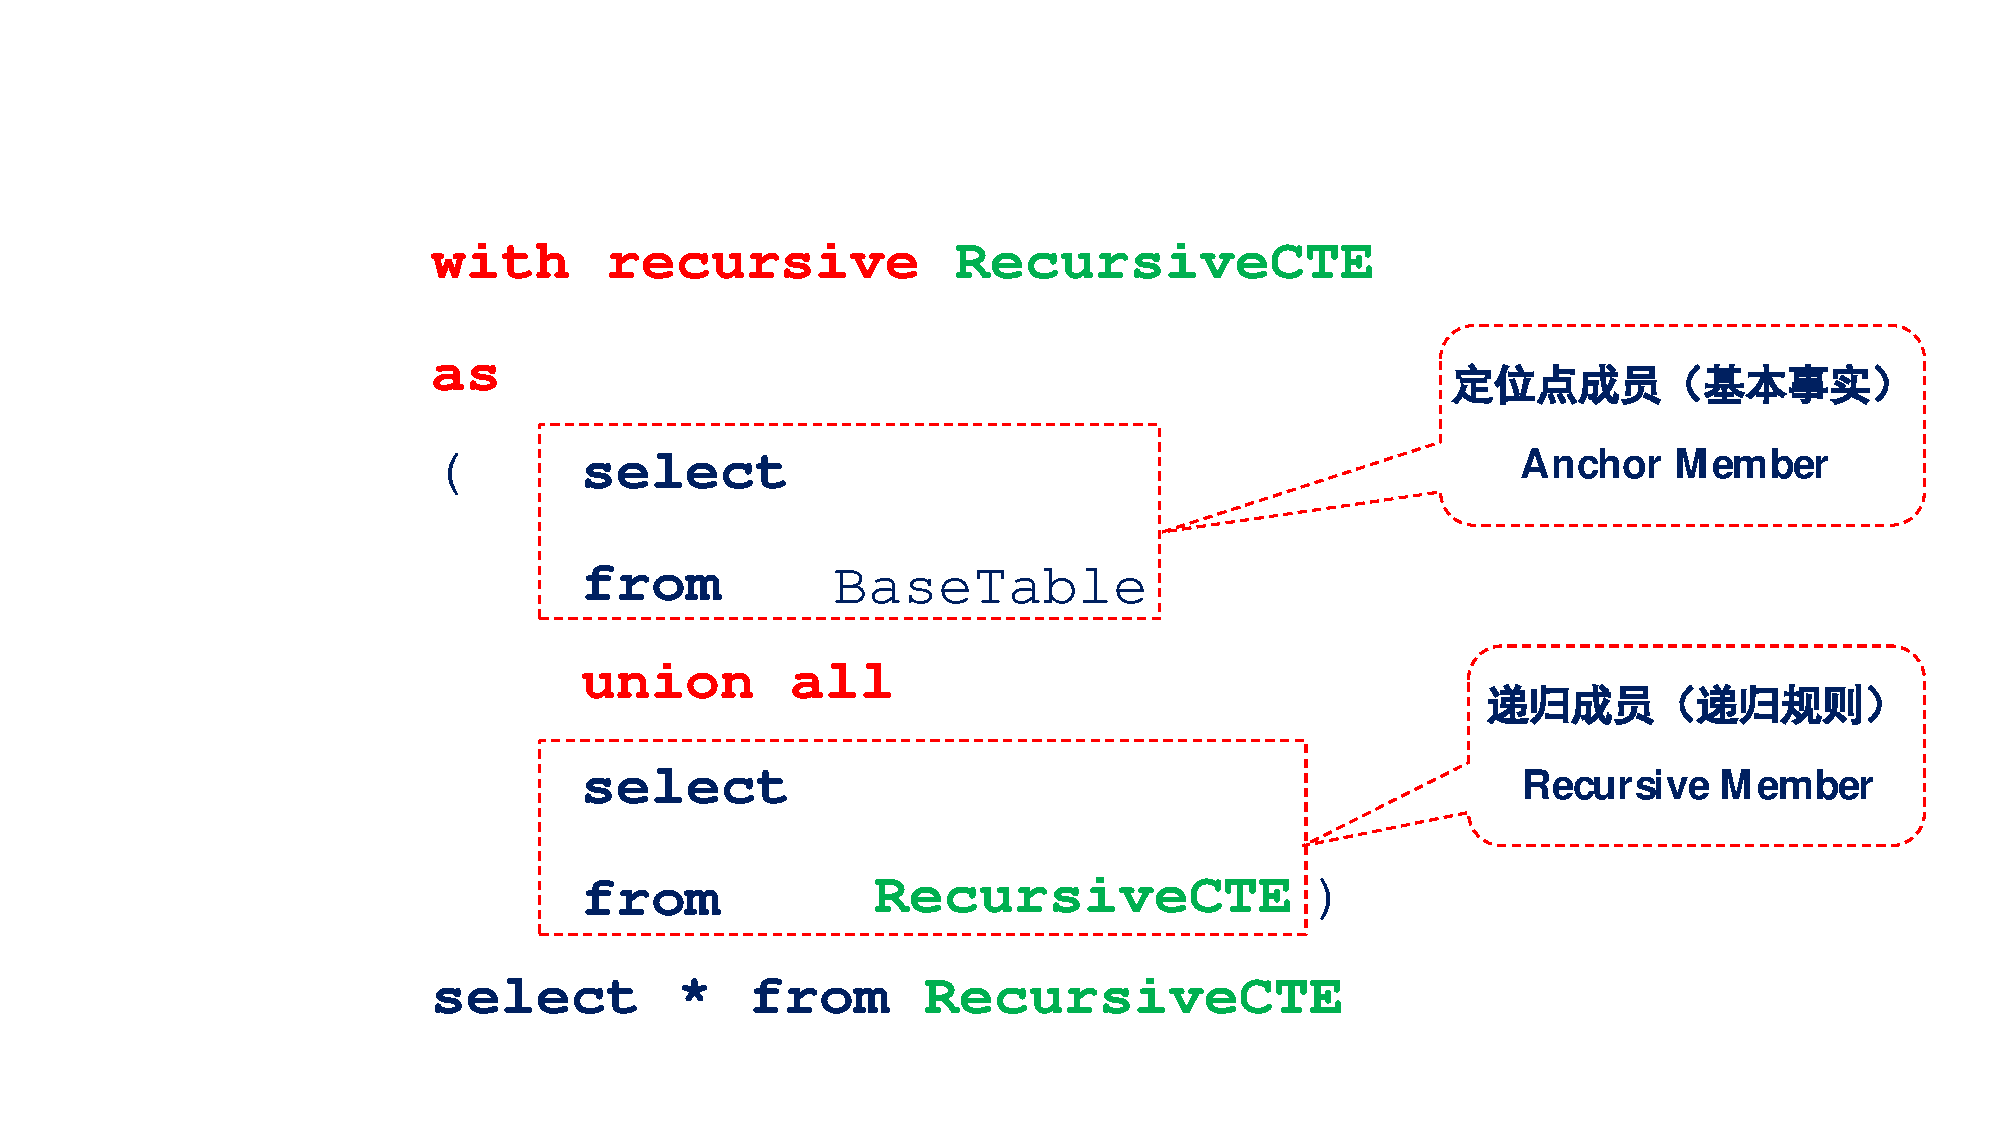
\includegraphics[width=.4\textwidth]{./image/递归查询.pdf}
    \caption{MySQL中的递归查询}
\end{figure}

\begin{lstlisting}[language=SQL]
with recursive nums(n)
as
(   select 1
    union all
    select n+1
    from nums
    where n < 100 )
select sum(n) from nums
\end{lstlisting}

\begin{lstlisting}[language=SQL]
with recursive Components ( part, subpart )
as
( select part, subpart
  from Assembly
  union all
  select A.part, C.subpart
  from Assembly A, Components C
  where A.subpart = C.part )
  select * from Components where part = 'trike'
\end{lstlisting}

\begin{example}
    利用递归查询计算经理下属. 表结构: emp(empid, ename, mgrid).
\end{example}

\begin{lstlisting}[language=SQL]
declare @root = 1 as int
-- 定义递归起点编号
with recursive SubsCTE
as ( select empid, ename, 0 as lvl
     from emp
     where empid = @root
     -- 初始查询
     union all
     select C.empid, C.ename, P.lvl + 1
     from SubsCTE as P join emp AS C on C.mgrid = P.empid
     -- 查询当前层级的表: SubsCTE
      )
select * from SubsCTE    
\end{lstlisting}

\begin{lstlisting}[language=SQL]
declare @lvl = 0 as int
create temporary table Subs( empid int, level int )
-- 插入根节点
insert into Subs( empid, level )
    select empid, @lvl from emp
    where empid = @root;
while found_rows() > 0

-- 递归查找下属
begin
    set @lvl = @lvl + 1
    insert into Subs( empid, level )
        select C.empid, @lvl
        from Subs as P join emp as C
        on P.lvl = @lvl - 1 and C.mgrid = P.empid
end    
\end{lstlisting}

\begin{figure}[H]
    \centering
    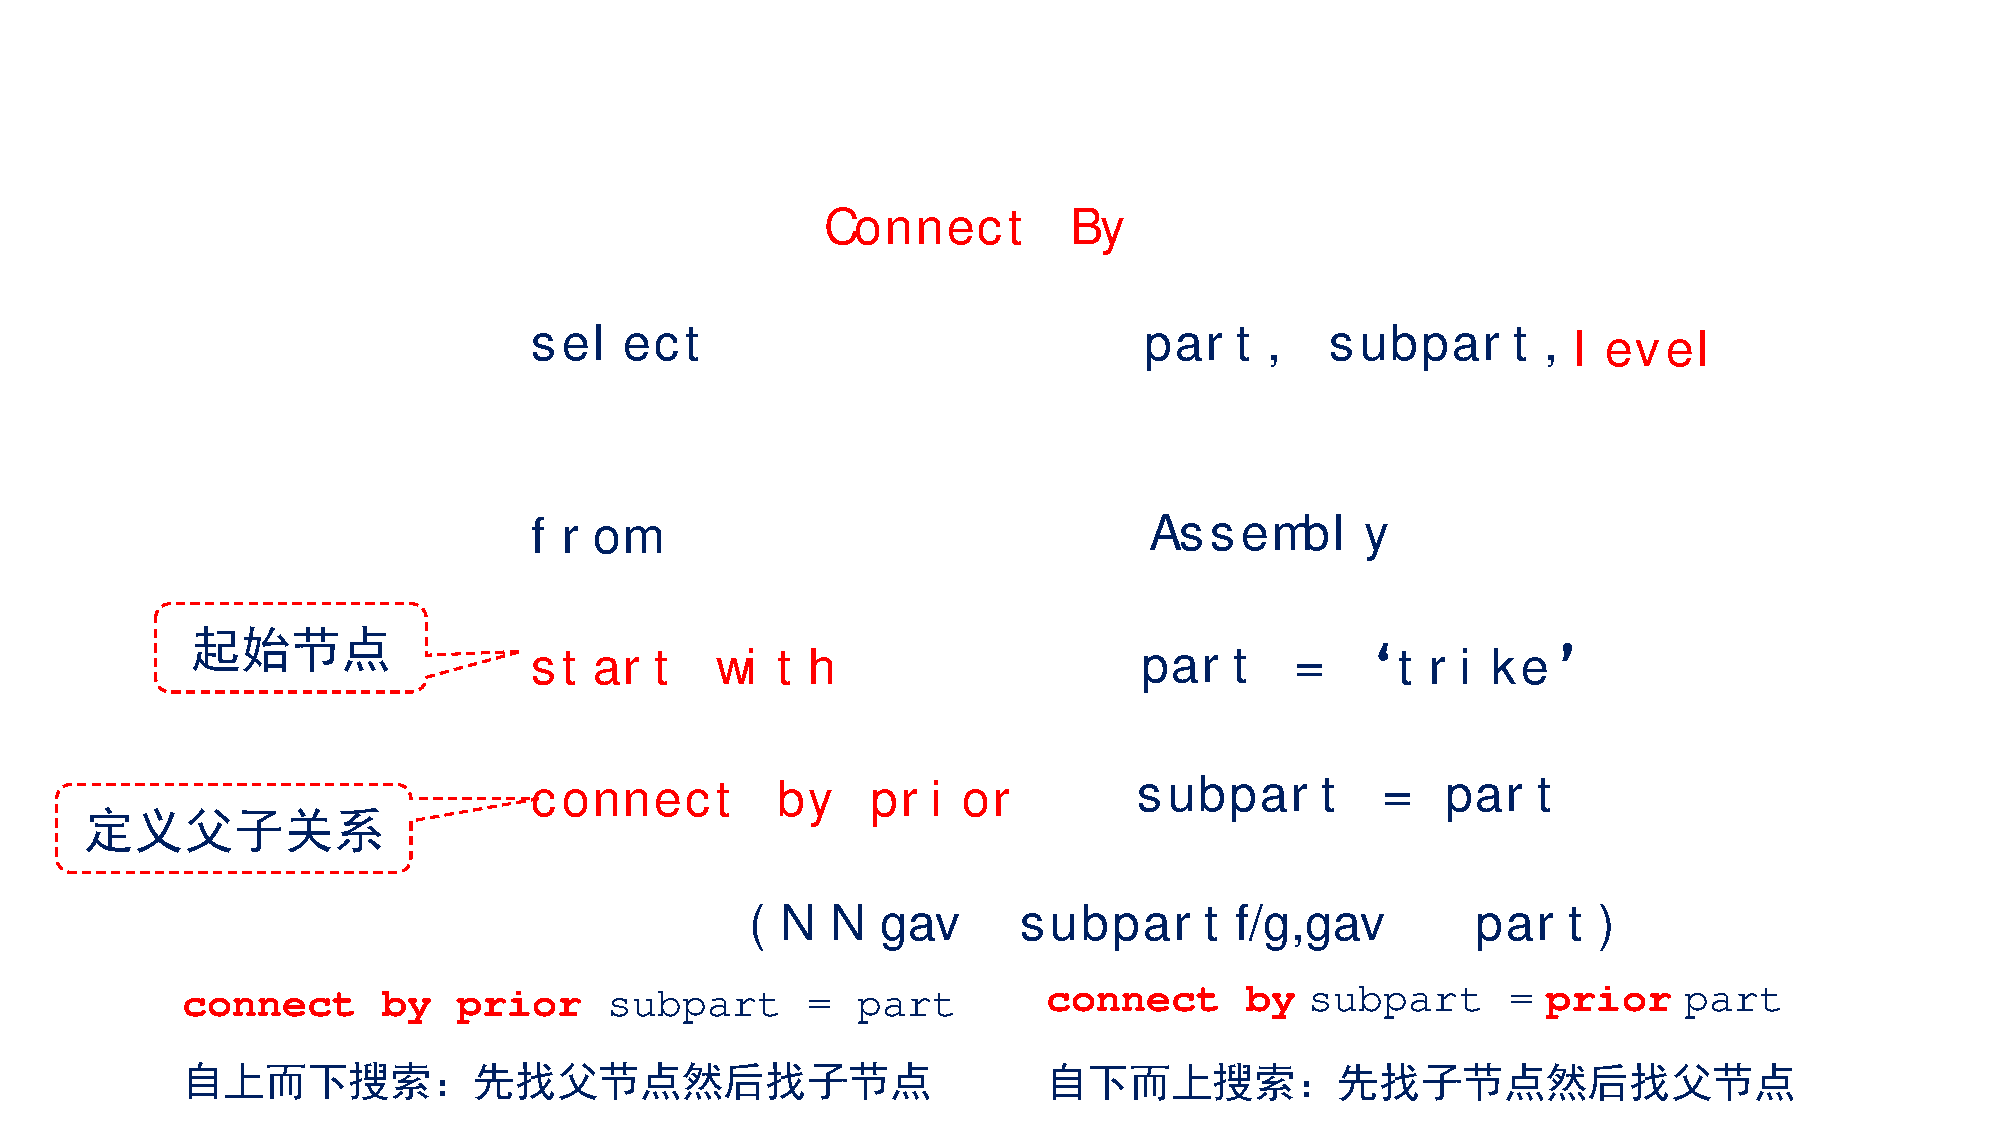
\includegraphics[width=.6\textwidth]{./figure/递归查询.pdf}
    \caption{Oracle中的递归查询}
\end{figure}

\subsection{层次结构典型查询问题}

树形结构(数据存放在邻接表中)
\begin{enumerate}
    \item 返回给定节点的所有下属,并标注层级
    \item 返回给定节点的所有上级,并标注层级
    \item 移动子树,将一颗子树的根节点换成另外一个
    \item 将邻接表转换为物化路径,并存放在一个表中
    \item 基于物化路径表,查询指定节点的所有子节点
    \item 基于物化路径表,查询指定节点的所有父节点
    \item 将邻接表转换为嵌套集合,并存放在一个表中
    \item 基于嵌套集合表,查询指定节点的所有子节点
    \item 基于嵌套集合表,查询指定节点的所有父节点
\end{enumerate}

图
\begin{enumerate}
    \item 计算传递闭包
    \item 计算最短路径
    \item 环路检测
\end{enumerate}

\section{XML}

\begin{enumerate}
    \item 标签(tag): 定义数据成为一个元素.
    \item 文本(text): 说明元素属性.
    \item 元素(elements): \texttt{<起始标签>元素属性<结束标签>}的组合.
\end{enumerate}

格式正确的(well-formed)XML文档
\begin{enumerate}
    \item 只能有唯一的根元素
    \item 所有元素都必须有起始标签和结束标签
    \item 大小写一致, XML区分大小写
    \item 子元素必须被上层元素完全包含
    \item 属性值必须被双引号或单引号括起来
    \item 元素内的属性不能被重复使用
\end{enumerate}

\begin{lstlisting}[language=XML]
<books>
    <book id="0001">
        <bookname> 数据库技术</bookname>
    </book>
    <book id="0001">
        <bookname> 数据仓库技术</bookname>
    </book>
</books>
\end{lstlisting}

HTML: HyperText Markup Language. 描述数据的显示格式

XML: eXtensible Markup Language. 描述数据的内容

XML: 半结构化模型的资源描述框架. RDF (Resource Description Framework)

存储RDF使用三元组: \texttt{<标识符, 属性名, 属性值>}. 或者\texttt{<Subject, Property, Object>}.

基于三元组表的RDF查询:
Implementation Techniques for Main Memory Databases喜欢什么和不喜欢什么?
\begin{lstlisting}[language=SQL]
SELECT    C.object, D.object
FROM      triples A, triples B, triples C, triples D
-- 四张相同的表triples, 别名分别为A, B, C, D
WHERE     A.subject = B.object
  AND     A.property = "title"
  AND     A.object = "Implementation Techniques for Main Memory Databases"
  -- A中找到标题为给出标题的对象.
  AND     B.property = "authorOf"
  -- B中找到authorOf A找出的书, 也就是找出作者
  AND     B.subject = C.subject
  AND     C.property = "likes"
  -- C中找出这个作者喜欢的东西
  AND     C.subject = D.subject
  AND     D.property = "dislikes"
  -- D中找出这个作者不喜欢的东西
\end{lstlisting}

三元组的\textcolor{red}{单属性表}表示: 过于细碎, 导致太多的连接操作.

三元组的\textcolor{red}{宽表}表示: 太多列+稀疏.

DTD(Document Type Definition)是XML的核心机制之一, 用于定义XML文档的结构和规则.
它的主要作用是:
\begin{enumerate}
    \item 验证 XML 文档的合法性: 确保 XML 文档的元素、属性、内容等符合预定义的结构规则.
    \item 约束文档格式: 通过定义元素的嵌套关系、属性的取值范围等, 保证数据的一致性和正确性.
    \item 支持数据交换: 为不同系统之间共享数据提供统一的结构规范.
\end{enumerate}

\begin{lstlisting}[language=XML]
<?xml version="1.0" encoding="UTF-8"?>
<!DOCTYPE note [
    <!ELEMENT note (to,from,heading,body)>
    <!ELEMENT to (#PCDATA)>
    <!ELEMENT from (#PCDATA)>
    <!ELEMENT heading (#PCDATA)>
    <!ELEMENT body (#PCDATA)>
]>
<note>
    <to>Tove</to>
    <from>Jani</from>
    <heading>Reminder</heading>
    <body>Don't forget me this weekend!</body>
</note>
\end{lstlisting}

每个DTD规则表达式是一个有限状态自动机.
\begin{lstlisting}[language=XML]
<!ELEMENT books (book+)>
<!ELEMENT book (title, author+, year, price)>
<!ATTLIST book id ID #REQUIRED>
<!ELEMENT title (#PCDATA)>
<!ELEMENT author (#PCDATA)>
<!ELEMENT year (#PCDATA)>
<!ELEMENT price (#PCDATA)>
<!ENTITY company "MyPublisher">
\end{lstlisting}

XML数据模型(DOM, Document Object Model)是 W3C(万维网联盟)制定的一种标准接口规范, 
用于动态访问和操作 XML 或 HTML 文档的内容、结构和样式. 
它是通过将文档解析为树形结构(即 DOM 树), 并以对象的形式表示每个节点(如元素、属性、文本等), 
从而允许程序或脚本以编程方式操作文档.

XPath (XML Path Language)是一种用于在 XML 或 HTML 文档中定位和选择节点的查询语言.
它通过路径表达式(Path Expressions)和条件筛选(谓语)来导航 XML 文档的树形结构, 
从而提取特定的数据或节点.


\begin{table}[H]
    \centering
    \begin{tabular}{|l|l|l|}
    \hline
    \textbf{表达式} & \textbf{含义} & \textbf{示例} \\
    \hline
    / & 从根节点开始选取 & /bookstore/book \\
    \hline
    // & 从当前节点开始,选取文档中任意位置的节点 & //title \\
    \hline
    . & 当前节点 & .//price \\
    \hline
    .. & 父节点 & ../author \\
    \hline
    @ & 选取属性 & @id \\
    \hline
    \end{tabular}
    \caption{路径表达式}
\end{table}

\begin{table}[H]
    \centering
    \begin{tabular}{|l|l|l|}
    \hline
    \textbf{表达式} & \textbf{含义} & \textbf{示例} \\
    \hline
    * & 选取所有子节点 & /* (根节点的所有子元素) \\
    \hline
    @* & 选取所有属性 & //@lang \\
    \hline
    text() & 选取文本节点 & //price/text() \\
    \hline
    \end{tabular}
    \caption{节点选择}
\end{table}

谓语(条件筛选):
\begin{itemize}
    \item \textbf{索引筛选}: [n] 选择第 n 个节点(从 1 开始计数):
    \begin{verbatim}
/bookstore/book[1]  % 第一个 book 节点
    \end{verbatim}
    \item \textbf{属性筛选}: [@属性名='值']:
    \begin{verbatim}
//book[@id='b001']  % id 为 b001 的 book 节点
    \end{verbatim}
    \item \textbf{文本筛选}: [text()='值'] 或 contains(text(), '部分值'):
    \begin{verbatim}
//title[text()='XML权威指南']  % 文本完全匹配
//title[contains(text(), '指南')]  % 文本包含 "指南"
    \end{verbatim}
\end{itemize}

\begin{table}[H]
    \centering\begin{tabular}{|l|l|l|}
        \hline
        \textbf{轴} & \textbf{含义} & \textbf{示例} \\
        \hline
        child:: & 子元素(默认可省略) & child::book (等价于 book) \\
        \hline
        parent:: & 父节点 & parent::bookstore \\
        \hline
        ancestor:: & 所有祖先节点 & ancestor::bookstore \\
        \hline
        descendant:: & 所有后代节点 & descendant::title \\
        \hline
        following-sibling:: & 所有后续兄弟节点 & following-sibling::author \\
        \hline
    \end{tabular}
    \caption{轴(Axis)}
\end{table}


MySQL中的XML函数: \verb|ExtractValue(xml_target, xpath_expr)|, 从 XML 数据中提取特定节点的值.
\begin{lstlisting}[language=SQL]
-- 提取 <to> 节点的值
SELECT ExtractValue('<note><to>Tove</to></note>', '/note/to');
-- 结果: Tove

-- 提取多个节点的值(使用 `|` 分隔)
SELECT ExtractValue('<a><b>1</b><c>2</c></a>', '//b/text() | //c/text()');
-- 结果: 1 2
\end{lstlisting}

\section{JSON}

JSON的基本成分为:
\begin{enumerate}
    \item 对象. \verb|{属性名: 属性值, 属性名: 属性值}|. E.g., \verb|{'name': 'Tom', 'hobby': ['sing', 'dance']}|.
    \item 数组. \verb|[value, value, value ...]|. \verb|[{'name': 'Tom', 'age': 12}, {...}]|.
\end{enumerate}

MySQL中生成JSON的函数:
\begin{enumerate}
    \item \texttt{JSON\_ARRAY} 函数. 创建一个 JSON 数组.
    \begin{verbatim}
JSON_ARRAY(val1, val2, ..., valN)
    \end{verbatim}
    \begin{verbatim}
SELECT JSON_ARRAY(1, 'apple', NULL, TRUE);
-- 输出: [1, "apple", null, true]
    \end{verbatim}
    \item \texttt{JSON\_OBJECT} 函数. 将键值对列表返回为JSON对象.
    \begin{verbatim}
JSON_OBJECT('key1' VALUE val1, 'key2' VALUE val2, ...)
    \end{verbatim}
    \begin{verbatim}
SELECT JSON_OBJECT('id' VALUE 1, 'name' VALUE 'Alice');
-- 输出: {"id": 1, "name": "Alice"}
    \end{verbatim}
\end{enumerate}

MySQL中的JSON数据类型:
\begin{lstlisting}[language=SQL]
CREATE TABLE testJSON (
    a JSON,
    b INT
);
INSERT INTO testJSON VALUES
('[3, 10, 5,"x", 44]', 33),
('[3, 10, 5, 17,[22,"y", 66]]', 0);
-- 提取嵌套值
SELECT a->"$[3]", a->"$[4][1]" FROM testJSON;
-- 结果分别为: ["x", 17], [NULL, "y"]
\end{lstlisting}

JSON的检索操作:
\begin{lstlisting}[language=SQL]
create table user (
    id int not null primary key auto_increment,
    info json );
insert into user(info) values (
    '{"name":"wangming",
      "age":18,
      "address":{"province":"sichuan","city":"chengdu"},
      "hobby" :["sing", "dance"]}' );

-- 提取多层嵌套值
SELECT json_extract('[10, 20, [30, 40]]', '$[2][*]');
-- 输出: [30, 40]

-- 提取 JSON 对象中的字段
SELECT json_extract(info, '$.address.city') FROM user;
-- 输出: "chengdu"

-- 提取多个字段
SELECT json_extract(info, '$.name', '$.hobby') FROM user;
-- 输出: ["wangming", ["sing", "dance"]]
\end{lstlisting}

将JSON展开为平面表:
\begin{lstlisting}[language=SQL]
-- 展开 JSON 数组为行
SELECT *
FROM json_table(
    '[{"a":"3"},{"a":2},{"b":1},{"a":0},{"a":[1,2]}]',
    "$[*]"
    COLUMNS(
        rowid FOR ORDINALITY,
        ac VARCHAR(100) PATH "$.a" DEFAULT '111' ON EMPTY DEFAULT '999' ON ERROR,
        aj JSON PATH "$.a" DEFAULT '{"x": 333}' ON EMPTY,
        bx INT EXISTS PATH "$.b"
    )
) AS tt;
\end{lstlisting}
上面展开后的结果为:
\begin{table}[H]
    \centering
    \begin{tabular}{|l|l|l|l|}
        \hline
        rowid & ac & aj & bx \\ \hline
        1 & 3 & "3" & 0 \\ \hline
        2 & 2 & 2 & 0 \\ \hline
        3 & 111 & \{"x": 333\} & 1 \\ \hline
        4 & 0 & 0 & 0 \\ \hline
        5 & 999 & [1, 2] & 0 \\ \hline
    \end{tabular}
\end{table}

将JSON展开为平面表: 数组的unwind操作.
\begin{lstlisting}[language=SQL]
-- 展开 JSON 中的嵌套数组(类似 unwind 操作)
SELECT *
FROM json_table(
    '[{"a": 1, "b": [11, 111]}, {"a": 2, "b": [22, 222]}, {"a": 3}]',
    "$[*]"
    COLUMNS(
        a INT PATH "$.a",
        NESTED PATH "$.b[*]" COLUMNS(b INT PATH "$")
    )
) AS jt
WHERE b IS NOT NULL;
\end{lstlisting}

将平面表转换为JSON:
\begin{lstlisting}[language=SQL]
-- 将平面表转换为 JSON 数组
CREATE TABLE score (
    sname CHAR(10),
    cname CHAR(10),
    score INT
);

INSERT INTO score VALUES
('张三', '数学', 96),
('张三', '语文', 99),
('李四', '数学', 98),
('李四', '语文', 88);

-- 转换为 JSON 数组
SELECT CONCAT(
    '[',
    GROUP_CONCAT(
        json_object('sname' VALUE sname, 'cname' VALUE cname, 'score' VALUE score)
    ),
    ']'
) AS scores
FROM score;
\end{lstlisting}

\section{向量}

向量嵌入使得我们具有处理非结构化数据的能力.

向量数据库中的核心问题: 近似最近邻查找. ANN (Approximate nearest neighbor search)

多维索引使用k-d tree: \href{https://oi-wiki.org/ds/kdt/}{k-d树文档}

近似最近邻搜索算法 ANNOY: \cite{liApproximateNearestNeighbor2016}.

高维数据的搜索: HNSW: Hierarchical Navigable Small World \cite{malkovEfficientRobustApproximate2018}.

基于PostgreSQL的向量插件: pgvector (基于IVFFlat索引), pg\_embedding (基于HNSW索引).
\begin{lstlisting}[language=SQL]
-- 1. 启用插件
CREATE EXTENSION vector;

-- 2. 创建表
CREATE TABLE items (
    id bigserial PRIMARY KEY,
    embedding vector(3)
);

-- 3. 插入数据
INSERT INTO items (embedding) VALUES
    ('[1,2,3]'),
    ('[4,5,6]');

-- 4. 创建索引(IVFFlat)
CREATE INDEX idx_items_embedding_ivfflat 
ON items 
USING ivfflat (embedding vector_l2_ops) 
WITH (lists = 100);

-- 5. 查询相似向量
SELECT * 
FROM items 
ORDER BY embedding <=> '[3,1,2]' 
LIMIT 5;
\end{lstlisting}